\documentclass[a4paper,12pt]{report}
\usepackage
[
a4paper,
left=4cm,
right=2.5cm,
top=3cm,
bottom=4cm,
]
{geometry}
\usepackage[czech]{babel}
\usepackage[utf8]{inputenc}
\usepackage[T1]{fontenc}
%\usepackage{hyperref}
\usepackage{xcolor} % barevný text - vyšedění
\usepackage{amsmath}
\usepackage{amssymb}
\usepackage{amsthm}
%\usepackage[toc,page]{appendix}
\usepackage{mdframed}
\usepackage{graphicx}
%\usepackage{subfigure}  % abych mohl dát 2 obrázky vedle sebe
\usepackage[font=footnotesize,labelfont=bf,justification=centering]{caption} % 2 obrázky vedle sebe, nastavuje font a centruje caption nad tabulkama a u obrázků
\usepackage[font=scriptsize]{subcaption}
\captionsetup{font=footnotesize}

%\usepackage{titlesec}
\usepackage{icomma} %nedělá za čárkou v číslech automaticky mezeru
\usepackage{url}
\usepackage{float}
\usepackage{enumerate} % hezky číslované listy (např. římská čísla)
%\usepackage[justification=centering]{caption} 

\usepackage{listings}
\usepackage{booktabs}

\newtheorem{theorem}{Věta}[chapter]
\newtheorem*{theoremnon}{Věta}
\newtheorem{lemma}{Lemma}[chapter]
\newtheorem{corollary}{Důsledek}[chapter]
%\theoremstyle{definition}
\newtheorem{definition}{Definice}[chapter]
\newtheorem*{defnon}{Definice}
\newtheorem{problem}{Úloha}[chapter]
\theoremstyle{remark}
\newtheorem{remark}{Poznámka}[chapter]

\renewcommand\qedsymbol{$\blacksquare$} % plný čtvereček za důkazem



\setlength{\topmargin}{-.25in}
\setlength{\parindent}{0pt}
\setlength{\parskip}{0.5\baselineskip}

%\usepackage{titlesec}
%\titleformat{\chapter}
%{\normalfont\LARGE}{\thechapter}{1em}{}
%\titlespacing*{\chapter}{0pt}{3.5ex plus 1ex minus .2ex}{2.3ex plus .2ex}

% Obecná definice pro styl nadpisů kapitol, sekcí atd. 
\usepackage{titlesec, blindtext, color}
\definecolor{gray75}{gray}{0.75}
\newcommand{\hsp}{\hspace{20pt}}

% Definice stylu pro chapter title
\titleformat{\chapter}[hang]{\Huge\bfseries}{\thechapter\hsp\textcolor{gray75}{|}\hsp}{0pt}{\Huge\bfseries}
% Definice stylu pro chapter title - bez číslování
\titleformat{name=\chapter,numberless}[hang]{\Huge\bfseries}{\hsp\textcolor{gray75}{|}\hsp}{0pt}{\Huge\bfseries}
% Definice stylu pro section title
\titleformat{\section}[hang]{\Large\bfseries}{\thesection\hsp\textcolor{gray75}{|}\hsp}{0pt}{\Large\bfseries}

\definecolor{identifiercolor}{rgb}{.4,.6,.56}
\definecolor{stringcolor}{gray}{0.5}
\definecolor{inactivecolor}{rgb}{0.15,0.15,0.5}
\usepackage{listings}
\lstset{basicstyle={\footnotesize\def\fvm@Scale{.85}\fontfamily{fvm}\selectfont},
	breaklines=true,
	escapeinside={\%*}{*)},
	keywordstyle={\bfseries\color{inactivecolor}},
	stringstyle={\bfseries\color{stringcolor}},
	identifierstyle={\bfseries\color{identifiercolor}},
	language=Mathematica,
	otherkeywords={DiscretizeRegion},
	showstringspaces=false}
\renewcommand{\lstlistingname}{Listing}


%%%%%%%% per partes
\ExplSyntaxOn
\NewDocumentCommand{\byparts}{O{0pt}m}
{
	\keys_set:nn { elisabeth/byparts } { #2 }
	\elisabeth_byparts:n { #1 }
}

\keys_define:nn { elisabeth/byparts }
{
	x  .tl_set:N = \l__elisabeth_byparts_u_tl,
	x' .tl_set:N = \l__elisabeth_byparts_up_tl,
	y  .tl_set:N = \l__elisabeth_byparts_v_tl,
	y' .tl_set:N = \l__elisabeth_byparts_vp_tl,
}

\cs_new_protected:Nn \elisabeth_byparts:n
{
	\begin{vmatrix}\,\begin{aligned}
			x\hphantom{'} &= \l__elisabeth_byparts_u_tl
			&
			y' &= \l__elisabeth_byparts_vp_tl
			\\[#1]
			x' &= \l__elisabeth_byparts_up_tl
			&
			y\hphantom{'} &= \l__elisabeth_byparts_v_tl
		\end{aligned}\,\end{vmatrix}
}

\ExplSyntaxOff
%%%%%%%%%%%%%%%%%


\title{
	{
\includegraphics[width=\linewidth]{FAV_logo.jpg}}\\[2cm]
	{Lineární řešiče v OpenFOAM}\\	
	{\small{Semestrální práce}}\\
	{\small{KMA/PVM}}\\
}

\author{Jan Půlpán}


\begin{document}
	\maketitle

	{\let\clearpage\relax \chapter{Teoretický úvod}}



	
	OpenFOAM je sada výpočetních nástrojů pro numerické simulace CFD (computational fluid dynamics) problémů, tedy problémů zabývajících se prouděním tekutin, vedením tepla a podobných procesů. OpenFOAM využívá k hledání řešení metody konečných objemů (FVM). My se budeme zabývat jen jednou částí celého řeťezce řešení problému a to sice popisem lineárních řešičů.
	
	FVM je numerická metoda na řešení parciálních diferenciálních rovnic na dané 3D geometrii převedené na síť nepřekrývajích se elementů (konečných objemů). Tu pak pomocí diskretizace převedeme na soustavu algebraických rovnich, kterou řešíme pomocí lineárních řešiců a výsledné řešení obsahuje hodnotu sledovaných proměnných pro každý z těchto elementů.
	
	Budeme se zabývat jen posledním článkem řetězce, tedy lineárními řešiči. Na testovací úloze si ukážeme vhodnost jednotlivých řešičů a budeme sledovat vliv parametrů na konvergenci řešení. Úkolem lineárních řešičů (dále budeme používat jen \uv{řešičů}, pokud nebude hrozit záměna kontextu) je najít řešení soustavy algebraických rovnic tvaru
	\begin{equation}
		\boldsymbol{A}x = b,
		\label{eq:linear_set}
	\end{equation}
	kde $\boldsymbol{A}$ je regulární matice popisující diskretizovaný model, $x$ vektor závislé proměnné a $b$ vektor pravé strany. 
	
	Pokud matice $\boldsymbol{A}$ umožňuje snadnou inverzi, je nejjednodušší získat přesné řešení soustavy přímým řešičem vztahem 
	$$ x = \boldsymbol{A}^{-1} b.$$ 
	Většinou ale nejde inverzi snadno nalézt a v tom případě se používají přibližné řešiče iterační. První variantou jsou stacionární iterační metody, kdy matici $\boldsymbol{A}$ můžeme rozdělit (například pomocí $LU$ rozkladu) na $\boldsymbol{A} = \boldsymbol{M} - \boldsymbol{N}$. matice $\pmb{M}$ musí být snadno invertovatelná a řešení pak hledáme poomocí iterací 
	
	\begin{equation}
		x^{(k+1)} = \boldsymbol{M}^{-1}(\boldsymbol{N}x^{(k)} + b)
		\label{eq:stat_iter}
	\end{equation}

	Pevný bod operátoru \eqref{eq:stat_iter} je pak přesným řešením soustavy \eqref{eq:linear_set}.  
	
	Druhou používanou metodou iteračních řešičů jsou metody Krylovových podprostorů. Hledáme tak přibližné řešení v podprostorech s rostoucí dimenzí generovaných čtvercovou maticí $\boldsymbol{A}$ a vektorem $\boldsymbol{b}$. Krylovův podprostor $r$tého řádu je definován jako 
	$$\mathcal{K}_r(\boldsymbol{A},\boldsymbol{b}) = \textrm{span}\{\boldsymbol{b}, \boldsymbol{Ab}, \boldsymbol{A}^2\boldsymbol{b}, \dots, \boldsymbol{A}^{r-1}\boldsymbol{b}\}.$$
	TROCHU LÍP POPSAT, KOUKNOUT DO NA
	
	Iterační metody obecně měří chybu aproximace řešení pomocí reziduí, tedy dosazením aproximovaného řešení do původních rovnic a vypočtením rozdílu oproti pravé straně $\boldsymbol{b}$. Reziduum $\boldsymbol{r}$ definujeme jako 
	\begin{equation}
		\boldsymbol{r} = \boldsymbol{b}-\boldsymbol{A}x.
		\label{eq:residuum}
	\end{equation} 
	
	
	Často se při numerickém řešení lineárních algebrických rovnic používá \textbf{předpodmínění}, které zajistí k rychlejší šíření informace na výpočetní mřížce. Při levém předpodmínění (existuje i pravé a centrální) Předpokládáme soustavu ve tvaru
	$$\boldsymbol{M}^{-1}\boldsymbol{A}x =\boldsymbol{M}^{-1}\boldsymbol{b}$$
	kde $\boldsymbol{M}$ je předpodmiňovač. Ten zajistí, že konvergence předpodmíněného systému je rychlejší, než bez něj. $\boldsymbol{M}$ je často uvažována jako snadno invertovatelná aproximace matice $\boldsymbol{A}$. Nejjednodušší volbou je tak $\boldsymbol{M} = \boldsymbol{I}$, což ovšem vede k nepodmíněnému problému. Ideální je naopak $\boldsymbol{M} = \boldsymbol{A}$, to ovšem znamená, že inverze předpodmiňovače je stejně náročná jako původní matice. JAK VYPADÁ ITERAČNÍ METODA - ZASE 
	

	
	SMOOTHER
	
	Although the preconditioners discussed before can considerably reduce the number of iterations, they do not normally reduce the mesh dependency of the numbers of iterations. OpenFOAM supplies the following smoothers to be used with the solvers in the smoothers/ directory:
	
	These smoothers are discussed in Section 9. For now, it suffices to view them as basic iterative methods (e.g. Gauss-Seidel) which effectively smooth out the error associated with
	the current approximate solution
	
	


	{\let\clearpage\relax \chapter{Lineární řešiče v OpenFOAM}}

OpenFOAM obsahuje kromě základního přímého řešiče \texttt{diagonalSolver} tři základní typy řešičů:
\begin{enumerate}
	\item řešiče metodou konjugovaných gradientů 
	\item smooth řešiče
	\item multigrid řešiče
\end{enumerate}

Jednotlivé řešiče jsou popsány v tabulce \ref{table:solvers}.

\begin{table}[H]
	\centering
	\caption{řešiče v rámci OpenFOAM}
	\renewcommand{\arraystretch}{1.7}
	\begin{tabular}{*3l}
		\toprule
		\textbf{Řešič} & \textbf{Označení}&\textbf{Matice $\boldsymbol{A}$}\\
		\midrule
		{\small Preconditioned conjugate gradient}& PCG& sym\\
		{\small Preconditioned bi-conjugate gradient}& PBiCG&asym \\		
		{\small Stabilized Preconditioned (bi-)conjugate gradient}& PBiCGStab&sym/asym  \\
		{\small Solver using a smoother}& smoothSolver&sym/asym \\
		{\small Generalised geometric-algebraic multi-grid}& GAMG&sym/asym  \\
		{\small Diagonal solver for explicit systems}& 	diagonal \\
	
		\bottomrule
	\end{tabular}
	
	\label{table:solvers}
\end{table}
		
To který řešič je možné použít je závislé na matici $\boldsymbol{A}$ a tom, jestli je symetrická nebo nesymetrická. Symetrie $\boldsymbol{A}$ samozřejmě závisí na rovnicích, které chceme řešit. V případě, že zvolíme nesprávný řešič vzhledem k symetričnosti matice $\boldsymbol{A}$ OpenFOAM sám volbu opraví.

Reziduum je během jednotlivých iterací vyhodnocováno pomocí vztahu \eqref{eq:residuum}. Každý řešič má k reziduu trochu jíný přístup, obecně ale dochází k normalizaci a škálování rezidua vztahy

$$n = \sum \left( | \boldsymbol{A}x - \boldsymbol{A}\hat{x} | + | \boldsymbol{b} - \boldsymbol{A}\hat{x} | \right),$$
$$r = \frac{1}{n} \sum | \boldsymbol{b} - \boldsymbol{A}x |.$$ 

Pro každý typ řešice se nastaví parametr pro velikost rezidua (\texttt{tolerance}) a také relativní toleranci (\texttt{relTol}) pro poměr aktuálního rezidua v rámci jedné iterace a počátečního rezidua před začátkem iterace. Řešič se následně zastaví pokud je splněna alespoň jedna z těchto podmínek:
\begin{enumerate}
	\item reziduum je menší než nastavená \texttt{tolerance},
	\item relativní tolerance je menší než nastavená \texttt{relTol},
	\item je dosaženo nastaveného maximálního počtu iterací \texttt{maxIter}.
\end{enumerate}


Metoda sdružených gradientů (conjugent gradients) - PCG. PBiCG, PBiCGStab

Metoda sdružených gradientů (CG) je iterační algoritmus řešení soustav lineárních rovnic, který využívá sdružených směrů a vyžaduje symetrickou matici (postivně definitní) matici $\boldsymbol{A}$. Proto vznikla i metoda "bi-conjugate gradients" (dvojitých sdružených směrů), která pracuje s asymetrickými maticemi. OpenFoam obsahuje řešiče PCG a PBiCG s implementací těchto řešičů. Obě varianty jsou předpodmíňěné. Navíc je obsažen i PBiCGStab řešič, který umí pracovat se symetricvkou i nesymetrickou maticí $\boldsymbol{A}$.

Předpodmičovač je volitelný a obsahuje následující možnosti:

Preconditioner	Keyword
Diagonal incomplete-Cholesky (symmetric)	DIC
Faster diagonal incomplete-Cholesky (DIC with caching)	FDIC
Diagonal incomplete-LU (asymmetric)	DILU
Diagonal	diagonal
Geometric-algebraic multi-grid	GAMG
No preconditioning	none



NĚCO O SMOOTH ŘEŠIČÍCH 

The solvers that use a smoother require the smoother to be specified. The smoother options are listed in Table 6.11. Generally GaussSeidel is the most reliable option, but for bad matrices DIC can offer better convergence. In some cases, additional post-smoothing using GaussSeidel is further beneficial, i.e. the method denoted as DICGaussSeidel


Smoother	Keyword
Gauss-Seidel	GaussSeidel
Diagonal incomplete-Cholesky (symmetric)	DIC
Diagonal incomplete-Cholesky with Gauss-Seidel (symmetric)	DICGaussSeidel





NĚCO O MULTIGRID ŘEŠIČÍCH (MULTIGRID METODY)

The generalised method of geometric-algebraic multi-grid (GAMG) uses the principle of: generating a quick solution on a mesh with a small number of cells; mapping this solution onto a finer mesh; using it as an initial guess to obtain an accurate solution on the fine mesh. GAMG is faster than standard methods when the increase in speed by solving first on coarser meshes outweighs the additional costs of mesh refinement and mapping of field data. In practice, GAMG starts with the mesh specified by the user and coarsens/refines the mesh in stages. The user is only required to specify an approximate mesh size at the most coarse level in terms of the number of cells nCoarsestCells.


NĚCO O RESIDUAL CONTROL

By default, cases will run until the time settings are achieved in the case controlDict dictionary. Alternatively, the residualControl object can be added to the fvSolution dictionary to enable additional controls. This operates in two modes:

Steady state
To terminate the case when the initial residual of the field equations falls below user-specified threshold values for SIMPLE-based solvers:

residualControl
{
	p           1e-2;
	"(Ux Uy)"   1e-4;
	"(k|epsilon|omega)" 1e-4;
}


NĚCO O RELAXACI

under-relaxation, a technique used for improving stability of a computation, particularly in solving steady-state problems. Under-relaxation works by limiting the amount which a variable changes from one iteration to the next, either by modifying the solution matrix and source prior to solving for a field or by modifying the field directly. An under-relaxation factor $\alpha, 0 < \alpha \leq 1$  specifies the amount of under-relaxation, ranging from none at all for $\alpha = 1$  and increasing in strength as $\alpha -> 0$ The limiting case where $\alpha =  0$  represents a solution which does not change at all with successive iterations. An optimum choice of $\alpha$  is one that is small enough to ensure stable computation but large enough to move the iterative process forward quickly; values of $\alpha$   as high as 0.9 can ensure stability in some cases and anything much below, say, 0.2 are prohibitively restrictive in slowing the iterative process


\begin{enumerate}
	\item jaké jsou možnosti, jaké jsou parametry
	\begin{enumerate}
		\item     diagonalSolver - pokud je matic A diagonální, pak vypočítám $A^{-1} = A/diag(A)$ a jsem hotov (https://www.openfoam.com/documentation/guides/latest/doc/guide-solvers.html)
	\end{enumerate}
\end{enumerate}





	{\let\clearpage\relax \chapter{Porovnání řešičů}}
	
	Lineární řešiče porovnáme na konkrétní úloze stacionárního proudění v lopatkové mříži. Zachováme přitom jednotné parametry nastavení úlohy až na nastavení jednotlivých lineárních řešičů. Zajímat nás bude konvergence řešení a výpočetní náročnost. Zadání úlohy je na obrázku \ref{fig:zadani}, který definuje geometrii úlohy i okrajové podmínky. 
	
	Používáme: simpleFoam - Steady-state solver for incompressible, turbulent flows
	
	\begin{figure}[H]
		\centering
		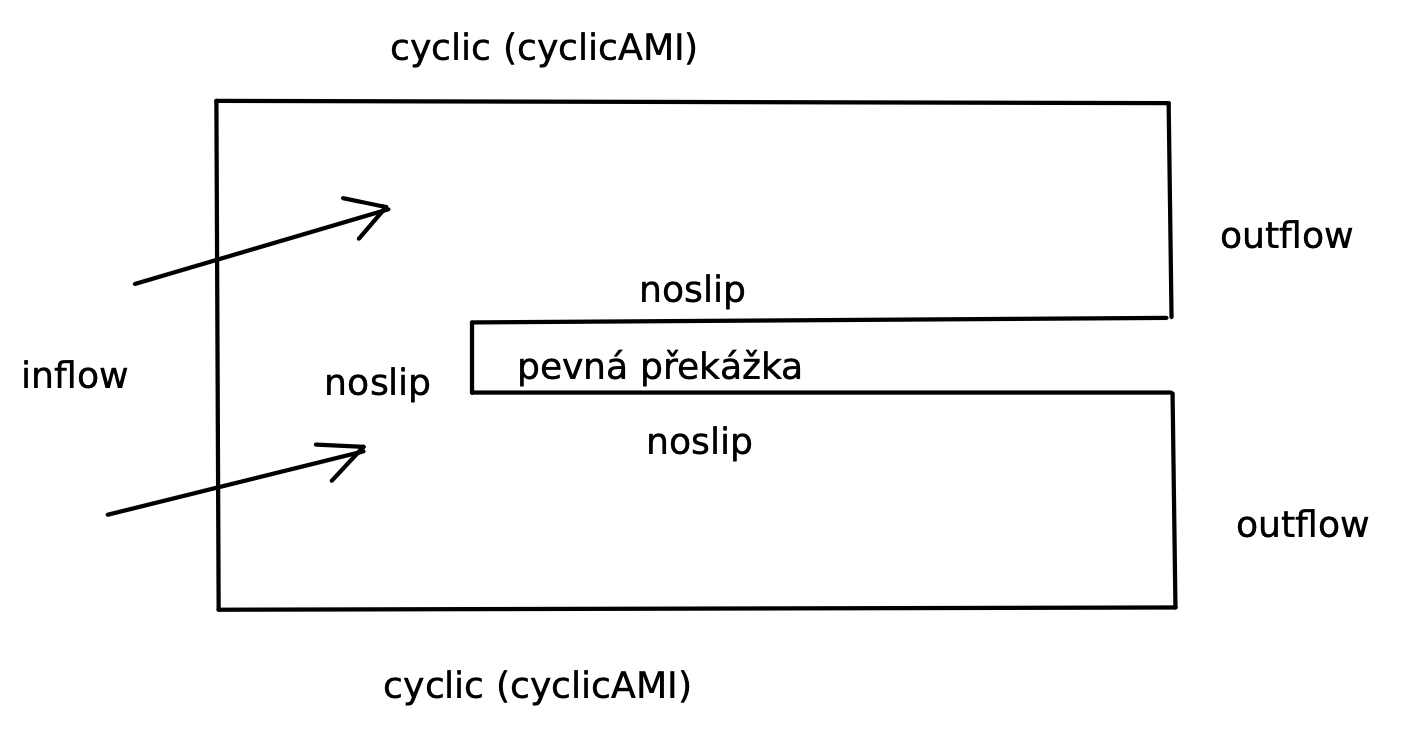
\includegraphics[width=1\linewidth]{zadani.png}
		\caption{Popis řešeného modelu}
		\label{fig:zadani}
	\end{figure}


Nejprve musíme definovat síť na které budeme naši úlohu řešit. .... Nadefinovaná síť je na obrázku \ref{fig:pvmesh}, konkrétní definice v přiloženém souboru \texttt{blockMeshDict}.

PŘIDAT OBRÁZKY S DETAILAMA OKOLO TOHO VYKOUSNUTÍ, UKÁZAT, ŽE TO JE NEHOMOGENNÍ, SPOČÍTAT KOLIK JE TAM VLASTNĚ TĚCH POLÍČEK

\begin{figure}[H]
	\centering
	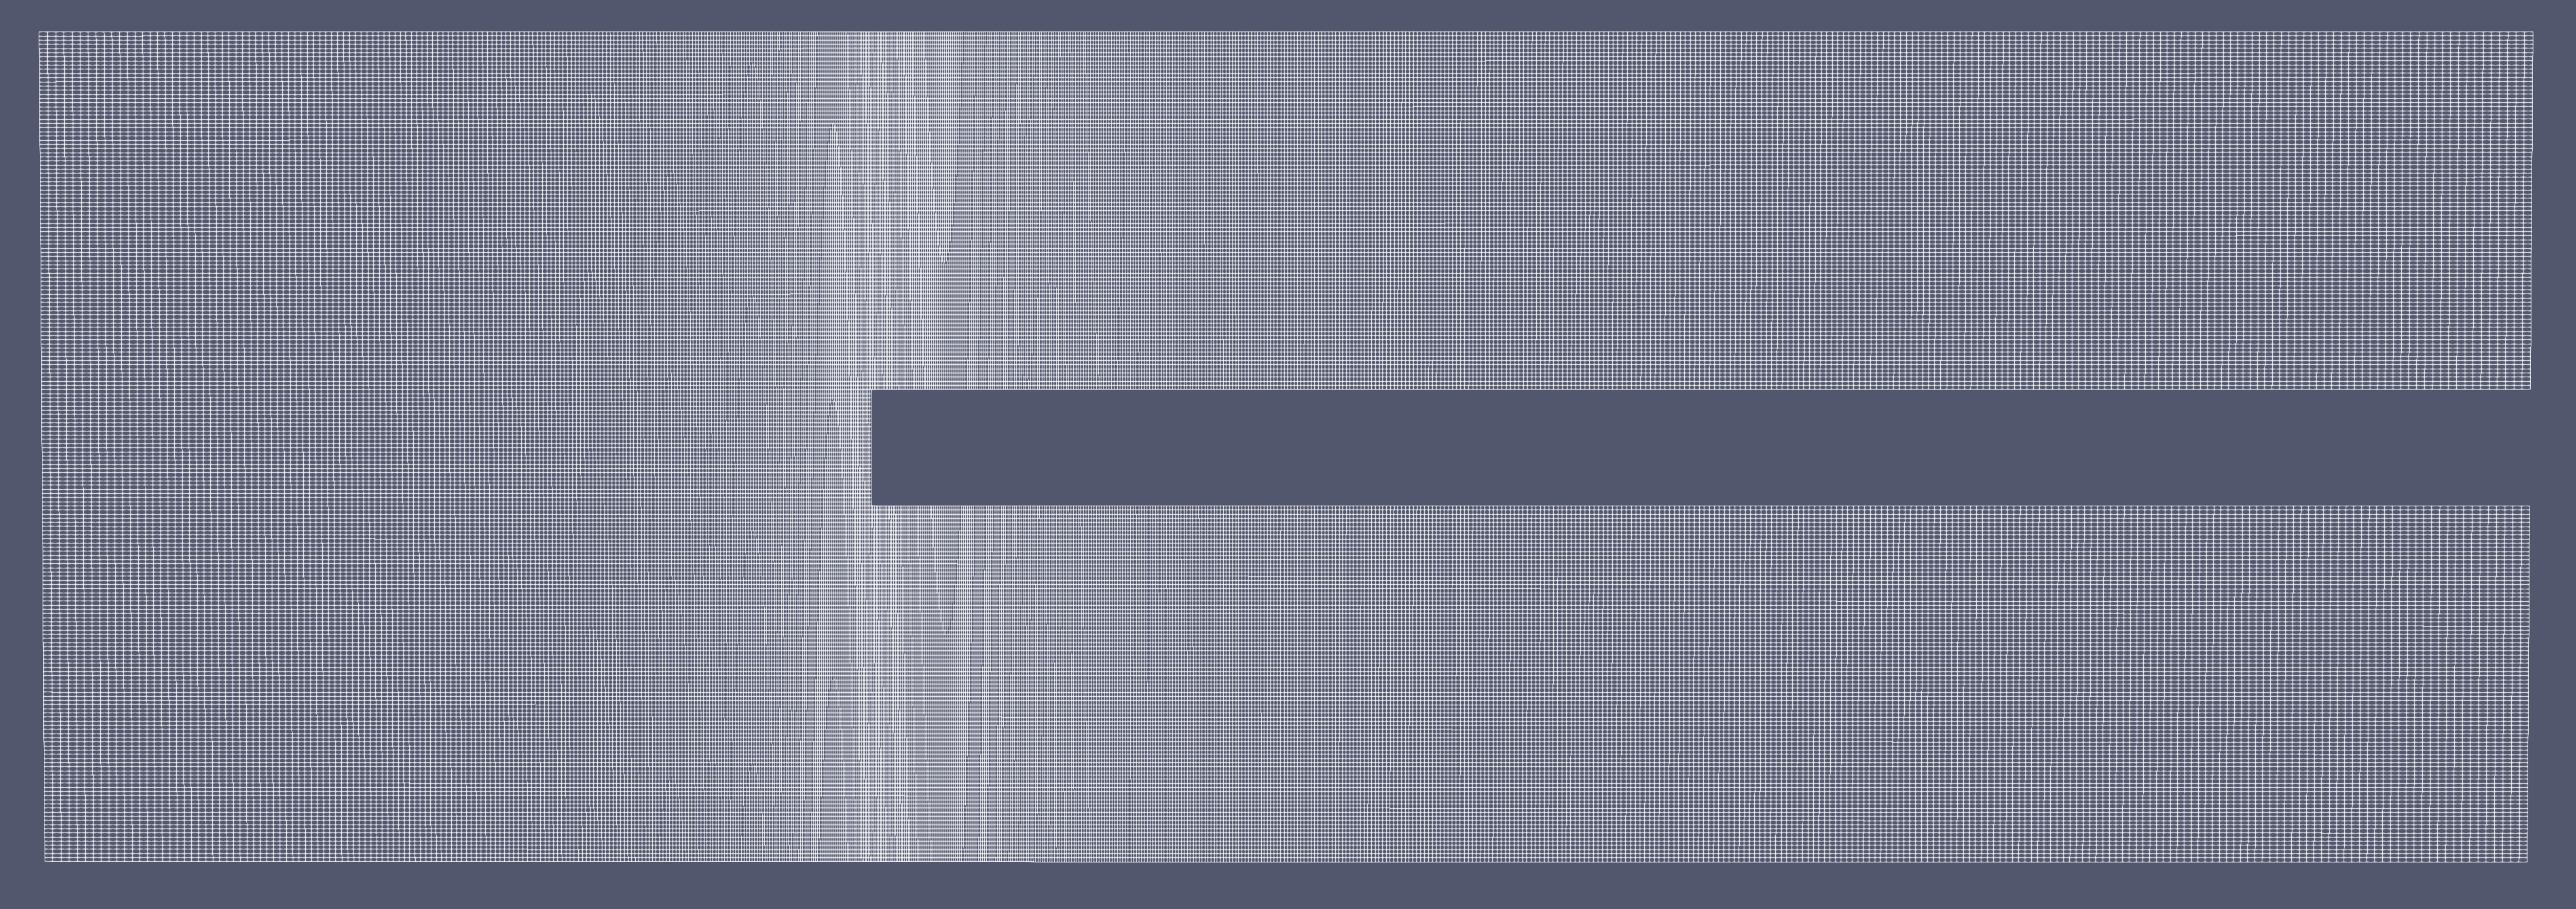
\includegraphics[width=1\linewidth]{pv-mesh.png}
	\caption{Síť řešeného modelu}
	\label{fig:pvmesh}
\end{figure}


Okrajové podmínky pro jednotlivé veličiny, pro nás primárně pro rychlost $U$ a tlak $p$  jsou definovány v souborech ve složce \texttt{0}.

Ostatní parametry řešiče úlohy, netýkající se přímo lineárních řešičů jsou pro všechny simulace totožné a jsou v souborech \texttt{transportProperties}, \texttt{turbulenceProperties}, \texttt{fvSchemes} a \texttt{controlDict}. Zde uvedeme jen vybrané parametry popisující naší úlohu.

\begin{itemize}
	\item{\makebox[5cm]{application\hfill}simpleFoam}
	\item{\makebox[5cm]{simulationType\hfill}RAS}
	\item{\makebox[5cm]{RASmodel\hfill}kEpsilon}
	\item{\makebox[5cm]{turbulence\hfill}on}
	\item{\makebox[5cm]{transportModel\hfill}Newtonian}
	\item{\makebox[5cm]{nu\hfill}1e-05}
\end{itemize}


	
Na ukázku je zde obrázek \ref{fig:pv-GAMG-GS} výsledného klidového stavu pořízený v ParaView. Výsledky úlohy řešené pomocí různých lineárních řešičů vypadají identicky.
	
	 \begin{figure}[H]
		\centering
		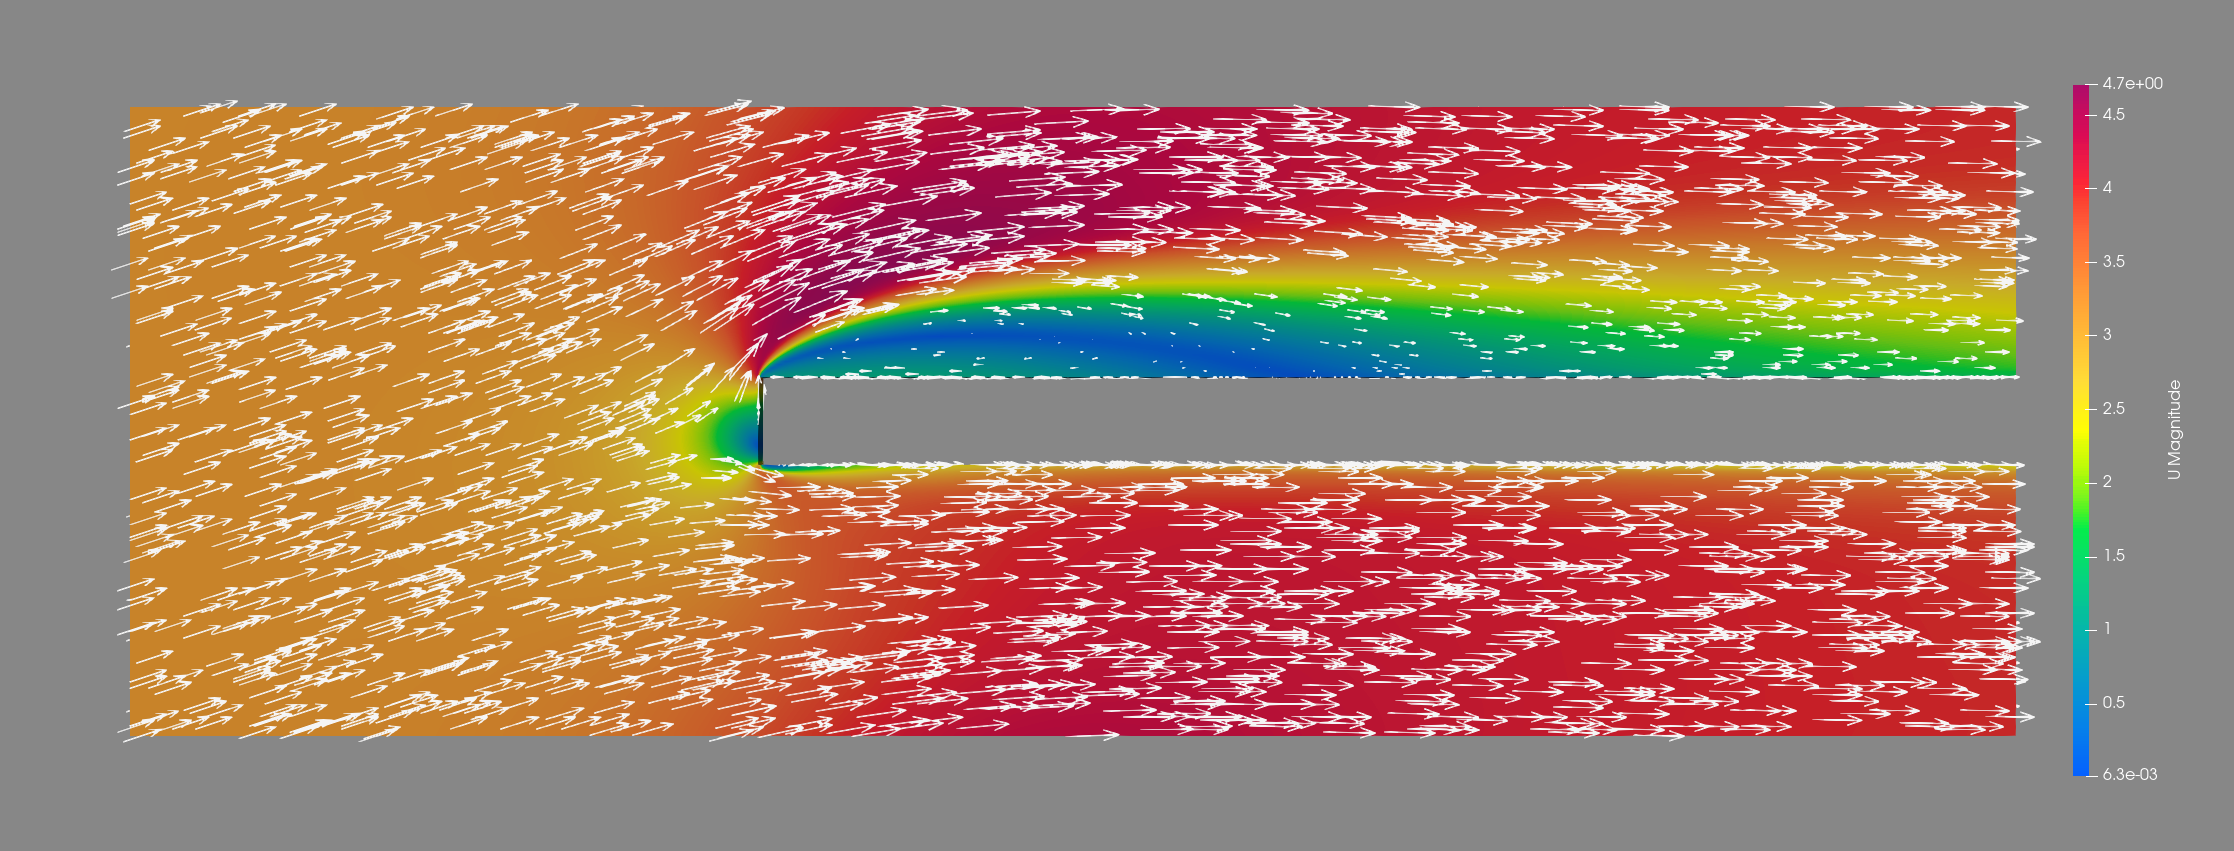
\includegraphics[width=1\linewidth]{pv-GAMG-GS.png}
		\caption{Klidový stav s vektory rychlosti $U$ v ParaView}
		\label{fig:pv-GAMG-GS}
	\end{figure}


Na lineárních řešičích budeme zkoumat vliv následujících parametrů na konvergenci simulace:
 
\begin{itemize}
	\item typ použitého řešiče
	\item typ použitého předpodmiňovače
	\item typ použitého smootheru
	\item pod-relaxace
\end{itemize}

Nastavení řešičů se v OpenFOAM dělá v souboru system/fvSolution. Ukázkový soubor je v příloze \ref{app:fvsol}.
	
 Nejprve nás zajímá typ použitého řešiče, případně přidruženého předpodmiňovače nebo smootheru. V tabulkách \ref{table:solvers_GAMG}, \ref{table:solvers_PCG} a \ref{table:solvers_smooth} jsou uvedená nastavení a výsledné počty iterací řešení úlohy a čas běhu simulace testovací úlohy.
 
 Konvergenci metody měříme pomocí počtu využitých iterací metody. Maximální počet iterací byl nastaven na $500$. Tolerance lineárního řešiče je shodně nastavena na $10^{-6}$, relativní tolerance na $0$. Velikost reziduí v rámci SIMPLE algoritmu pomocí \texttt{residualControl} parametru pro tlak $p$ nastaveno na $10^{-3}$ a pro rychlost $U$ na $10^{-4}$.

 \begin{table}[H]
	\centering
	\caption{Nastavení lineárních řešičů pro jednotlivé simulace}
	\renewcommand{\arraystretch}{1.9}
	\begin{tabular}{*7c}
		\toprule
		%\multicolumn{2}{c}{\textbf{Řešič pro $p$}} & \multicolumn{2}{c}{\textbf{Řešič pro $U$}}\\
		\multicolumn{2}{c}{Tlak $p$: \textbf{GAMG}} & \multicolumn{2}{c}{Rychlost $U$: \textbf{GAMG}}\\		
		\midrule
		%\textit{Předpod.}&\textit{Smoother}&\textit{Předpod.}&\textit{Smoother}&\textit{Relaxace}&\textit{ \# iter}&\textit{čas}\\
		Předpod.&Smoother&Předpod.&Smoother&\# iter&Čas\\
		\midrule
 --- & DIC & --- &  DILU & 475 &157.94\\		
 --- & GaussSeidel &  --- & GaussSeidel & 475&176.99\\
		
			\bottomrule
\end{tabular}

\label{table:solvers_GAMG}

\end{table}


\begin{table}[H]
\centering
\caption{Nastavení lineárních řešičů pro jednotlivé simulace}
\renewcommand{\arraystretch}{1.9}
\begin{tabular}{*7c}
\toprule	

%\multicolumn{2}{c}{\textbf{}} & \multicolumn{2}{c}{\textbf{Řešič pro $U$}}\\
\multicolumn{2}{c}{Tlak $p$: \textbf{PCG}} & \multicolumn{2}{c}{Rychlost $U$: \textbf{PBiCG}}\\		
\midrule
%\textit{Předpod.}&\textit{Smoother}&\textit{Předpod.}&\textit{Smoother}&\textit{Relaxace}&\textit{ \# iter}&\textit{čas}\\
Předpod.&Smoother&Předpod.&Smoother&\# iter&Čas\\
\midrule
 DIC & --- &  DILU & --- &474&540.48\\								
FDIC & --- &  DILU & --- &474&531.14\\	
 \shortstack{GAMG\\GS smooth.}& --- &  \shortstack{GAMG\\GS smooth.}& --- &475&184.85\\	
diagonal & --- & diagonal & ---&474&679.26\\	

		\bottomrule
\end{tabular}

\label{table:solvers_PCG}

\end{table}

 \begin{table}[H]
	\centering
	\caption{Nastavení lineárních řešičů pro jednotlivé simulace}
	\renewcommand{\arraystretch}{1.9}
	\begin{tabular}{*7c}
		\toprule
\multicolumn{2}{c}{Tlak $p$: \textbf{smoothSolver}} & \multicolumn{2}{c}{Rychlost $U$: \textbf{smoothSolver}}\\
%\multicolumn{2}{c}{\textbf{Řešič pro $p$}} & \multicolumn{2}{c}{\textbf{Řešič pro $U$}}\\
%\multicolumn{2}{c}{\textbf{smoothSolver}} & \multicolumn{2}{c}{\textbf{smoothSolver}}\\		
\midrule
%\textit{Předpod.}&\textit{Smoother}&\textit{Předpod.}&\textit{Smoother}&\textit{Relaxace}&\textit{ \# iter}&\textit{čas}\\
Předpod.&Smoother&Předpod.&Smoother&\# iter&Čas\\
\midrule		
 --- & DIC &  --- & GaussSeidel &500+&1136.21\\	
 --- & DIC & --- & DILU &500+&1039.73\\
 --- & GaussSeidel &   --- & GaussSeidel &500+&1011.42\\		
 FDIC & GaussSeidel &  --- & GaussSeidel &500+&1008.47\\
 --- & \shortstack{symGauss-\\Seidel} &  --- & \shortstack{symGauss-\\Seidel}&500+&1370.58\\	
\bottomrule
\end{tabular}
	
	\label{table:solvers_smooth}
\end{table}


GAMG A PCG/PBiCG JSOU V POŘÁDKU. SMOOTH ALE ANI JEDEN NEDOBĚHL. PRŮBĚH JEDNOTLIVÝCH SIMULACÍ POMOCÍ VÝVOJE REZIDUA JE NA OBRÁZCÍCH XYZ (PRO P) A XZZ (PRO XOVOU SOUŘADCICI U). 

NEJLEPŠÍCH VÝSLEDKŮ DOSAHUJE GAMG ŘEŠIČ. - VÍME PROČ? - OBECNĚ ZNÁMÝ FAKT, SPECIÁLNĚ PRO P. GAMG NENÍ ALE TAK ŠKÁLOVATELNÝ JAKO PCG/PBICG A TAK JE MOŽNÉ, ŽE PROP JINOU A SLOŽITEJŠÍ ÚLOHU BY MOHLO BÝT PCG VHODNĚJŠÍ.

\begin{figure}[H]
	\centering
	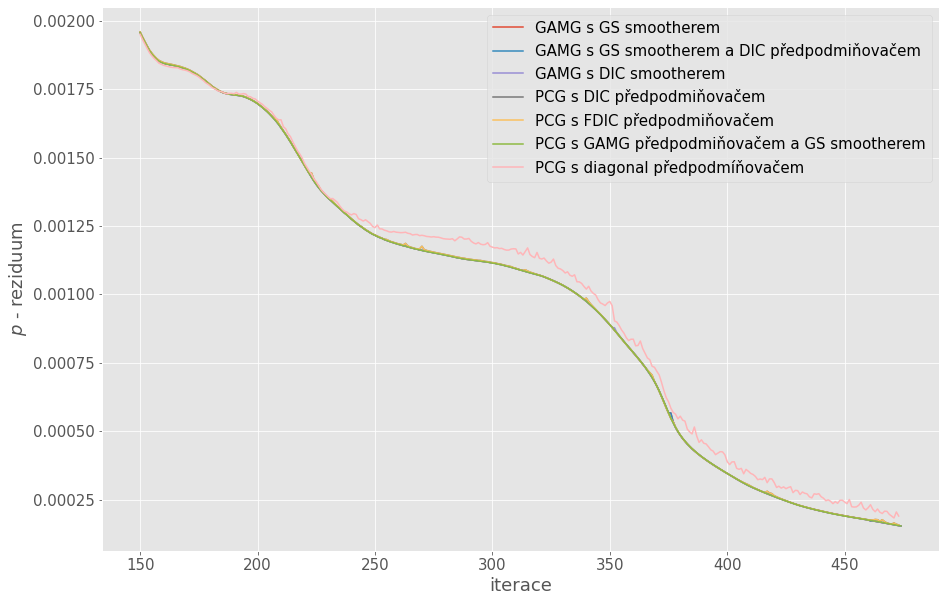
\includegraphics[width=1\linewidth]{p-residuum.png}
	\caption{Konvergence lineárních řešičů v různé konfiguraci pro tlak $p$}
	\label{fig:p-residuum}
\end{figure}


\begin{figure}[H]
	\centering
	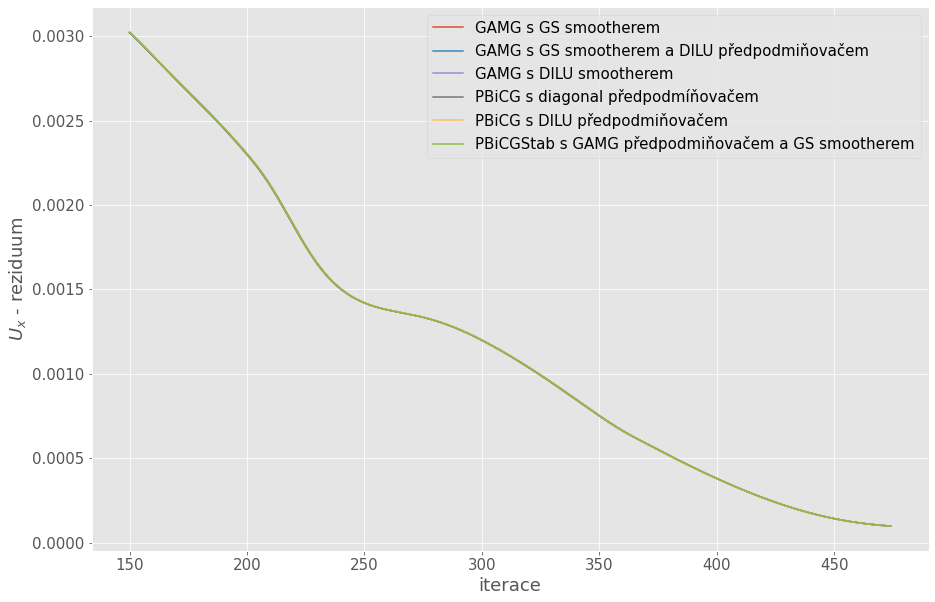
\includegraphics[width=1\linewidth]{ux-residuum.png}
	\caption{Konvergence lineárních řešičů v různé konfiguraci pro rychlost $U_x$}
	\label{fig:ux-residuum}
\end{figure}

NA OBRÁZCÍCH ASD A BNM JE VIDĚT PROBLÉM SE SMOOTH ŘEŠIČI. N EJEN ŽE JSOU EXTRÉMNĚ POMALÉ, ALE JEŠTĚ K TOMU NEJSOU SCHPNY V NASTAVENÉM POČTU MAXITER DOKONVERGOVAT. POPSAT OSCILACE A ŽE JDOU PROTI SOBĚ. KDYŽ NAJDU DŮVOD NEVHODNOSTI SMOOTH ŘEŠIČE, TAK DOPSAT.

\begin{figure}[H]
	\centering
	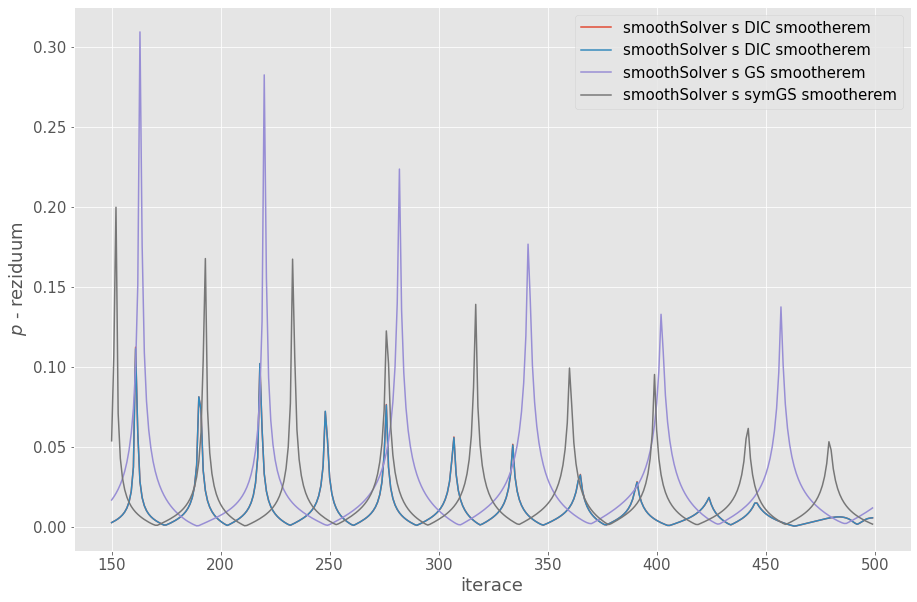
\includegraphics[width=1\linewidth]{p-residuum-smooth.png}
	\caption{Konvergence lineárních řešičů smoothSolver v různé konfiguraci pro tlak $p$}
	\label{fig:p-residuum-smooth}
\end{figure}

\begin{figure}[H]
	\centering
	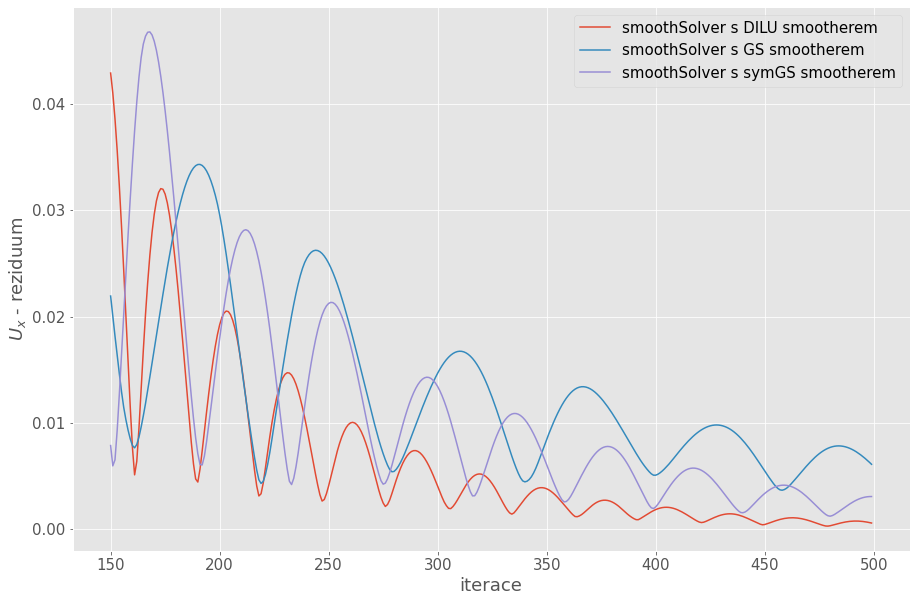
\includegraphics[width=1\linewidth]{ux-residuum-smooth.png}
	\caption{Konvergence lineárních řešičů smoothSolver v různé konfiguraci pro rychlost $U_x$}
	\label{fig:ux-residuum-smooth}
\end{figure}
	

DÁLE NÁS BUDE ZAJÍMAT POD-RELAXACE (VYSVĚTLENÍ JE JIŽ NAHOŘE) PRIMÁRNĚ U GAMG. V TABULCE HJK JSOU VÝSLEDKY. UŽ TADY OKOMENTOVAT.

 \begin{table}[H]
	\centering
	\caption{Nastavení lineárních řešičů pro jednotlivé simulace}
	\renewcommand{\arraystretch}{1.9}
	\begin{tabular}{*8c}
		\toprule
		\multicolumn{2}{c}{Tlak $p$: \textbf{GAMG}} & \multicolumn{2}{c}{Rychlost $U$: \textbf{GAMG}}\\		
		\midrule
		%\textit{Předpod.}&\textit{Smoother}&\textit{Předpod.}&\textit{Smoother}&\textit{Relaxace}&\textit{ \# iter}&\textit{čas}\\
		Předpod.&Smoother&Předpod.&Smoother&Relaxace& \# iter&Čas\\
		
		\midrule
		
		--- & GaussSeidel &  --- & GaussSeidel & 0.9&475&176.99\\
		--- & GaussSeidel &  --- & GaussSeidel & 0.3&500+&151.49\\
		--- & GaussSeidel &  --- & GaussSeidel & 0.95&285&114.15\\
		--- & GaussSeidel &  --- & GaussSeidel & 0.98&500+&257.28\\		
		DIC & GaussSeidel &  DILU & GaussSeidel & 0.98&475&160.59\\
		\bottomrule
	\end{tabular}
	
	\label{table:solvers_gamg_relax}
	
\end{table}

NA OBRÁZCÍCH X A Y JE OPĚT PRŮBĚH REZIDUA. Z NICH JE VIDĚT NESTABILITA .98 RELAXACE JAK V P TAK V U

\begin{figure}[H]
	\centering
	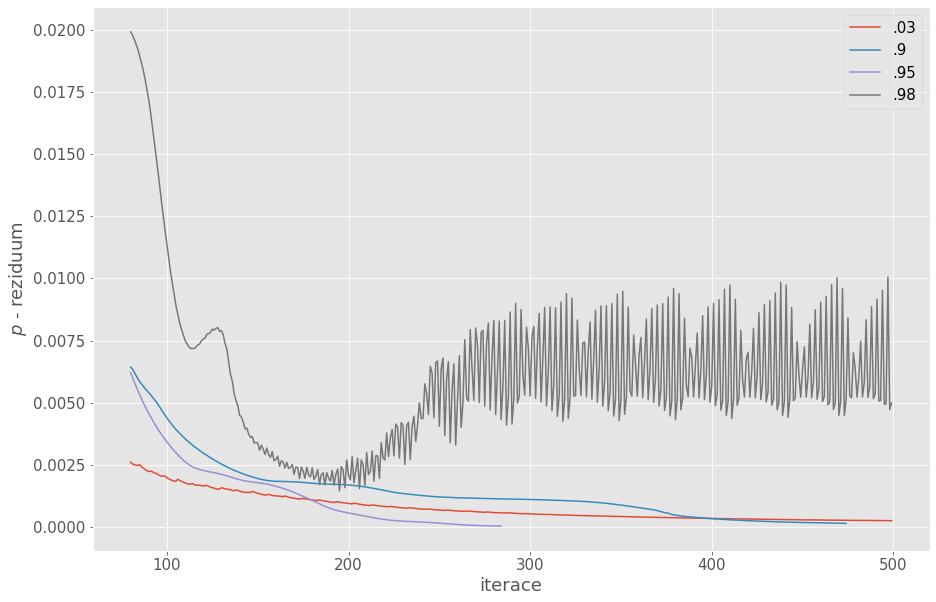
\includegraphics[width=1\linewidth]{p-under-relax.png}
	\caption{Konvergence lineárních řešičů smoothSolver v různé konfiguraci pro rychlost $U_x$}
	\label{fig:p-residuum-relax}
\end{figure}

\begin{figure}[H]
	\centering
	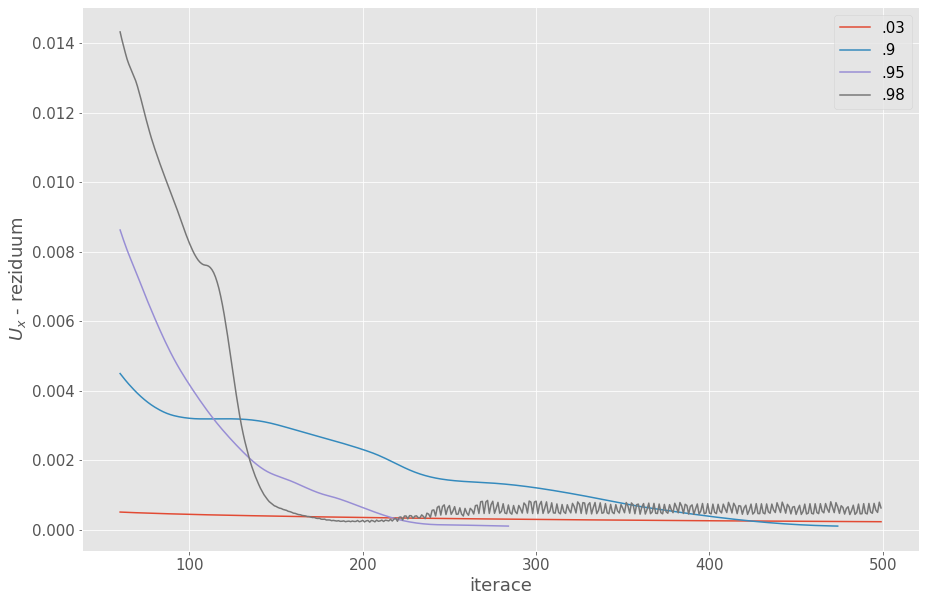
\includegraphics[width=1\linewidth]{ux-under-relax.png}
	\caption{Konvergence lineárních řešičů smoothSolver v různé konfiguraci pro rychlost $U_x$}
	\label{fig:ux-residuum-relax}
\end{figure}

POKUS POUŽÍT UNDERRELAX U SMOOTH NEVYŠEL, VÝSLEDKY LEPŠÍ NEJSOU

\begin{table}[H]
	\centering
	\caption{Nastavení lineárních řešičů pro jednotlivé simulace}
	\renewcommand{\arraystretch}{1.9}
	\begin{tabular}{*8c}
		\toprule
		\multicolumn{2}{c}{Tlak $p$: \textbf{smoothSolver}} & \multicolumn{2}{c}{Rychlost $U$: \textbf{smoothSolver}}\\
		\midrule
		%\textit{Předpod.}&\textit{Smoother}&\textit{Předpod.}&\textit{Smoother}&\textit{Relaxace}&\textit{ \# iter}&\textit{čas}\\
		Předpod.&Smoother&Předpod.&Smoother&Relaxace& \# iter&Čas\\
		\midrule
		--- & GaussSeidel &   --- & GaussSeidel &0.9&500+&1011.42\\
		--- & GaussSeidel &  --- & GaussSeidel &0.3&500+&951.71\\
		--- & GaussSeidel &   --- & GaussSeidel &0.95&500+&1086.7\\
		--- & GaussSeidel &  --- & GaussSeidel &0.98&500+&1222.24\\
		FDIC & GaussSeidel &  --- & GaussSeidel &0.9&500+&1008.47\\
		\bottomrule
	\end{tabular}
	
	\label{table:solvers_set3}
\end{table}

ZAJÍMAVÝ JE TAKÉ VÝVOJ POČTU ITERACÍ JEDNOTLIVÝCH ŘEŠĚNÍ POMOCÍ LINEÁRNÍHO ŘEŠIČE - CO TO VLASTNĚ JE, JAK JE TO NASTAVENÉ, ATD - ZASE JE Z TOHO VIDĚT ŽE GAMG FUNGUJE NEJLÍP

\begin{figure}[H]
	\centering
	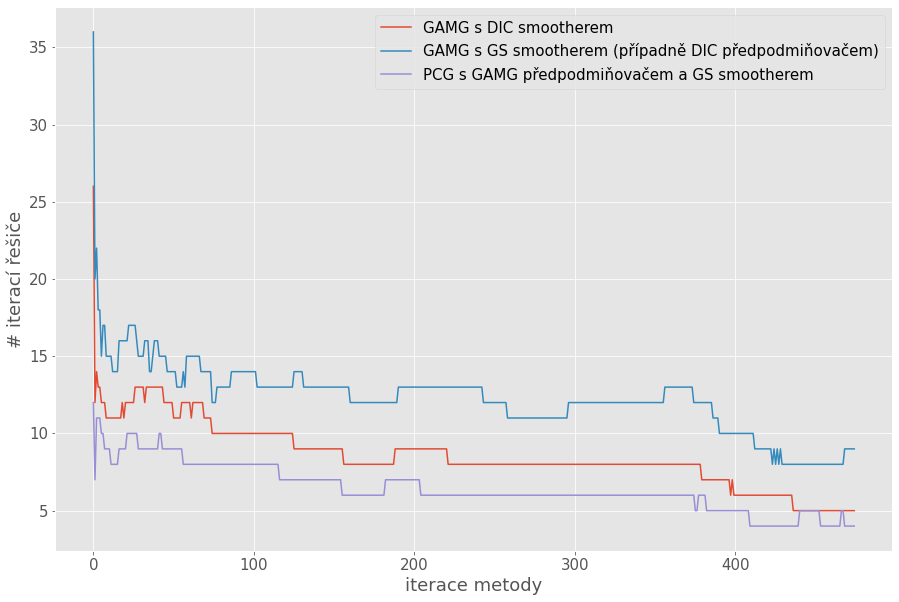
\includegraphics[width=1\linewidth]{p-solver-iters-1.png}
	\caption{Konvergence lineárních řešičů smoothSolver v různé konfiguraci pro rychlost $U_x$}
	\label{fig:p-iters-1}
\end{figure}

\begin{figure}[H]
	\centering
	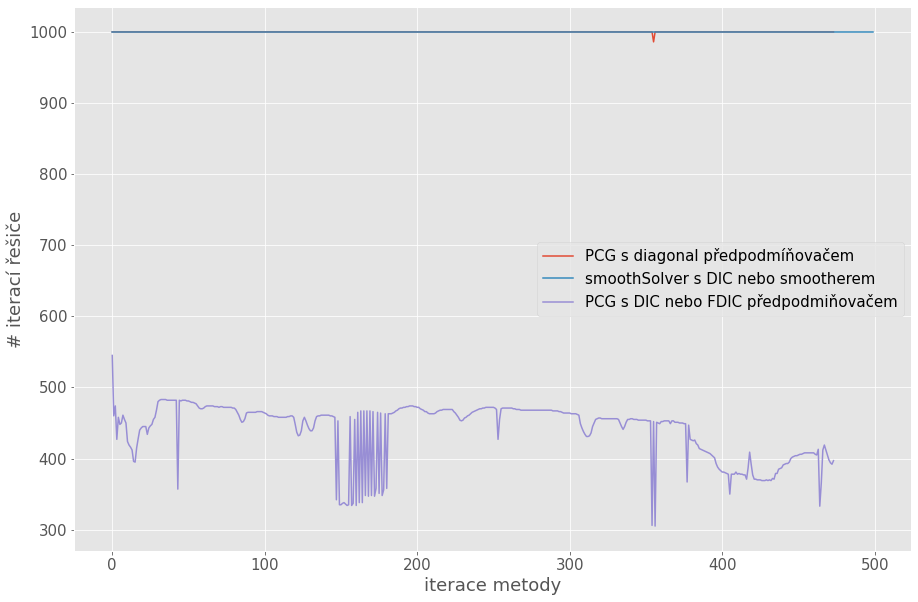
\includegraphics[width=1\linewidth]{p-solver-iters-2.png}
	\caption{Konvergence lineárních řešičů smoothSolver v různé konfiguraci pro rychlost $U_x$}
	\label{fig:p-iters-2}
\end{figure}

\begin{figure}[H]
	\centering
	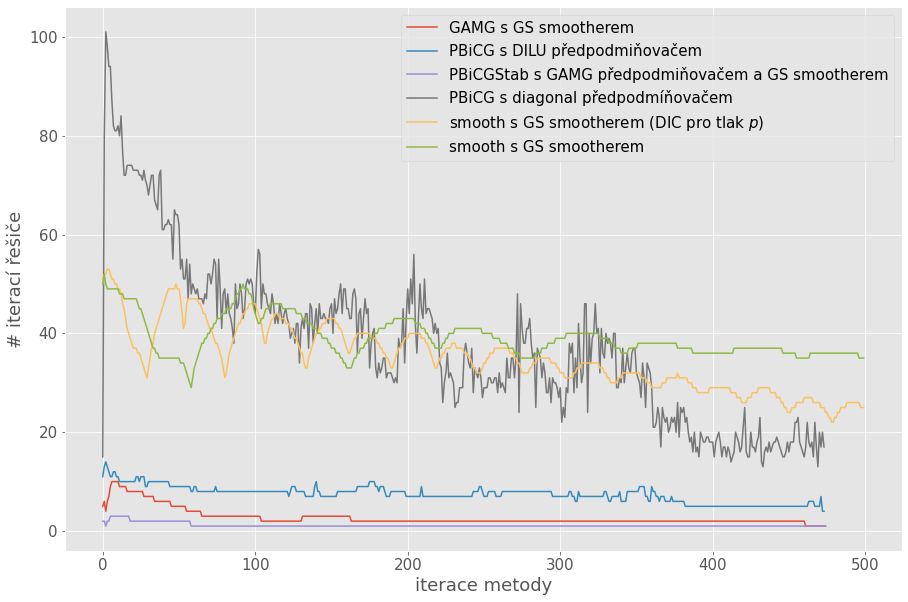
\includegraphics[width=1\linewidth]{ux-solver-iters.png}
	\caption{Konvergence lineárních řešičů smoothSolver v různé konfiguraci pro rychlost $U_x$}
	\label{fig:ux-iters}
\end{figure}



{\let\clearpage\relax \chapter{Závěr}}

Nelze dělat obecné závěry, volba řešiče vždy záleží na úloze, nastavených parametrech, tolerancích a třeba i hordwaru, který máme k dispozici. Jediný závěr, který tedy můžeme udělat se týká jen naší úlohy, pro kterou je nejvhodnější řešič XYZ.


 \begin{table}[H]
	\centering
	\caption{Nastavení lineárních řešičů pro jednotlivé simulace}
	\renewcommand{\arraystretch}{1.9}
	\begin{tabular}{*8c}
		\toprule
		\multicolumn{2}{c}{\textbf{Řešič pro $p$}} & \multicolumn{2}{c}{\textbf{Řešič pro $U$}}\\
		\multicolumn{2}{c}{\textbf{GAMG}} & \multicolumn{2}{c}{\textbf{GAMG}}\\		
		\midrule
		%\textit{Předpod.}&\textit{Smoother}&\textit{Předpod.}&\textit{Smoother}&\textit{Relaxace}&\textit{ \# iter}&\textit{čas}\\
		Předpod.&Smoother&Předpod.&Smoother&Relaxace& \# iter&Čas\\
		
		\midrule
		
		--- & DIC & --- &  DILU & 0.9&475 &157.94\\
		
		--- & GaussSeidel &  --- & GaussSeidel & 0.9&475&176.99\\
		
		--- & GaussSeidel &  --- & GaussSeidel & 0.3&500+&151.49\\
		
		--- & GaussSeidel &  --- & GaussSeidel & 0.95&285&114.15\\
		
		--- & GaussSeidel &  --- & GaussSeidel & 0.98&500+&257.28\\
		
		DIC & GaussSeidel &  DILU & GaussSeidel & 0.98&475&160.59\\
		\bottomrule
	\end{tabular}
	
	\label{table:solvers_set1}
	
\end{table}


\begin{table}[H]
	\centering
	\caption{Nastavení lineárních řešičů pro jednotlivé simulace}
	\renewcommand{\arraystretch}{1.9}
	\begin{tabular}{*8c}
		\toprule	
		
		\multicolumn{2}{c}{\textbf{Řešič pro $p$}} & \multicolumn{2}{c}{\textbf{Řešič pro $U$}}\\
		\multicolumn{2}{c}{\textbf{PCG}} & \multicolumn{2}{c}{\textbf{PBiCG}}\\		
		\midrule
		%\textit{Předpod.}&\textit{Smoother}&\textit{Předpod.}&\textit{Smoother}&\textit{Relaxace}&\textit{ \# iter}&\textit{čas}\\
		Předpod.&Smoother&Předpod.&Smoother&Relaxace& \# iter&Čas\\
		\midrule
		
		
		DIC & --- &  DILU & --- &0.9&474&540.48\\								
		
		FDIC & --- &  DILU & --- &0.9&474&531.14\\	
		
		\shortstack{GAMG\\GS smooth.}& --- &  \shortstack{GAMG\\GS smooth.}& --- &0.9&475&184.85\\	
		
		diagonal & --- & diagonal & --- &0.9&474&679.26\\	
		
		\bottomrule
	\end{tabular}
	
	\label{table:solvers_set2}
	
\end{table}

\begin{table}[H]
	\centering
	\caption{Nastavení lineárních řešičů pro jednotlivé simulace}
	\renewcommand{\arraystretch}{1.9}
	\begin{tabular}{*8c}
		\toprule
		
		\multicolumn{2}{c}{\textbf{Řešič pro $p$}} & \multicolumn{2}{c}{\textbf{Řešič pro $U$}}\\
		\multicolumn{2}{c}{\textbf{smoothSolver}} & \multicolumn{2}{c}{\textbf{smoothSolver}}\\		
		\midrule
		%\textit{Předpod.}&\textit{Smoother}&\textit{Předpod.}&\textit{Smoother}&\textit{Relaxace}&\textit{ \# iter}&\textit{čas}\\
		Předpod.&Smoother&Předpod.&Smoother&Relaxace& \# iter&Čas\\
		\midrule
		
		
		
		--- & DIC &  --- & GaussSeidel &0.9&500+&1136.21\\	
		
		--- & DIC & --- & DILU &0.9&500+&1039.73\\
		
		--- & GaussSeidel &   --- & GaussSeidel &0.9&500+&1011.42\\
		
		--- & GaussSeidel &  --- & GaussSeidel &0.3&500+&951.71\\
		
		--- & GaussSeidel &   --- & GaussSeidel &0.95&500+&1086.7\\
		
		--- & GaussSeidel &  --- & GaussSeidel &0.98&500+&1222.24\\
		
		FDIC & GaussSeidel &  --- & GaussSeidel &0.9&500+&1008.47\\
		
		--- & \shortstack{symGauss-\\Seidel} &  --- & \shortstack{symGauss-\\Seidel} &0.9&500+&1370.58\\	
		\bottomrule
	\end{tabular}
	
	\label{table:solvers_set3}
\end{table}






\newpage
\appendix
{\let\clearpage\relax \chapter{fvSolution}\label{app:fvsol}}
\begin{verbatim}
	/*---------------------------*- C++ -*-----------------------------*\
	| =========                 |                                                 |
	| \\      /  F ield         | OpenFOAM: The Open Source CFD Toolbox           |
	|  \\    /   O peration     | Version:  v2006                                 |
	|   \\  /    A nd           | Website:  www.openfoam.com                      |
	|    \\/     M anipulation  |                                                 |
	\*-----------------------------------------------------------------*/
	FoamFile
	{
		version     2.0;
		format      ascii;
		class       dictionary;
		location    "system";
		object      fvSolution;
	}
	// * * * * * * * * * * * * * * * * * * * * * * * * * * * * * * * * //
	
	solvers
	{
		p
		{
			solver          smoothSolver;
			smoother        GaussSeidel;
			tolerance       1e-06;
			relTol          0; 
		}
		
		"(U|k|epsilon|omega|f|v2)"
		{
			solver          smoothSolver;
			smoother        GaussSeidel;
			tolerance       1e-06;
			relTol          0; 
		}
	}
	
	SIMPLE
	{
		nNonOrthogonalCorrectors 0;
		consistent      yes;
		
		residualControl
		{
			p               1e-3;
			U               1e-4;
			"(k|epsilon|omega|f|v2)" 1e-4;
		}
	}
	
	relaxationFactors
	{
		equations
		{
			U               .95; 
			".*"            .95;
		}
	}
	
	
	// ************************************************************** //
\end{verbatim}
	
\end{document}